\subsection{Expression Class}
\label{sec:expression}

An \code{Expression} is an AST representation of how the value of an \code{Operand} is
computed/evaluated.

Evaluation attempts to determine the \code{Result} of the
computation that the AST being evaluated represents. It will fill in results of
as many of the nodes in the tree as possible, and if full evaluation is
possible, it will return the result of the computation performed by the tree.

Equality of two expressions, \code{E_1} and \code{E_2}, is defined by
\begin{itemize}
\item \code{E_1} and \code{E_2} are the same type
\item If leaf nodes, they represent the same immediate value or the same register
\item If non-\/leaf nodes, they represent the same operation and their corresponding children are equal 
\end{itemize}

\begin{apient}

Permissible leaf nodes of an \code{Expression} tree are RegisterAST and Immediate
objects. Permissible internal nodes are \code{BinaryFunction} and Dereference objects.
An \code{Expression} may represent an immediate value, the contents of a register, or
the contents of memory at a given address, interpreted as a particular type.

The \code{Result}s in an \code{Expression} tree contain a type and a value. Their values may
be an undefined value or an instance of their associated type. When two \code{Result}s
are combined using a \code{BinaryFunction}, the \code{BinaryFunction} specifies the output
type. Sign extension, type promotion, truncation, and all other necessary
conversions are handled automatically based on the input types and the output
type. If both of the \code{Result}s that are combined have defined values, the
combination will also have a defined value; otherwise, the combination's value
will be undefined. For more information, see
Section~\ref{sec:result}, Section~\ref{sec:binaryFunction}, and
Section~\ref{sec:dereference}.

A user may specify the result of evaluating a given \code{Expression}. This mechanism
is designed to allow the user to provide a Dereference or RegisterAST with
information about the state of memory or registers. It may additionally be used
to change the value of an Immediate or to specify the result of a
\code{BinaryFunction}. This mechanism may be used to support other advanced analyses.

In order to make it more convenient to specify the results of particular
subexpressions, the \code{bind} method is provided. \code{bind} allows the user
to specify that a given subexpression has a particular value everywhere that it
appears in an expression. For example, if the state of certain registers is
known at the time an instruction is executed, a user can \code{bind} those
registers to their known values throughout an \code{Expression}.

The evaluation mechanism, as mentioned above, will evaluate as many
sub-\/expressions of an expression as possible. Any operand that is more
complicated than a single immediate value, however, will depend on register or
memory values. The \code{Result}s of evaluating each subexpression are cached
automatically using the \code{setValue} mechanism. The \code{Expression} then attempts
to determine its \code{Result} based on the \code{Result}s of its children. If this \code{Result} can
be determined (most likely because register contents have been filled in via
\code{setValue} or \code{bind}), it will be returned from \code{eval}; if it can
not be determined, a \code{Result} with an undefined value will be returned. See Figure
6 for an illustration of this concept; the operand represented is 
\code{[ \code{EBX} + \code{4} $\ast$ \code{EAX} ]}. 
The contents of \code{EBX} and \code{EAX} have been determined through some
outside mechanism, and have been defined with \code{setValue}. The \code{eval}
mechanism proceeds to determine the address being read by the \code{Dereference}, since
this information can be determined given the contents of the registers. This
address is available from the Dereference through its child in the tree, even
though calling \code{eval} on the Dereference returns a \code{Result} with an
undefined value.

\dotfile deref-eval.dot
"Applying eval to a Dereference tree with the state of the registers known and the state of memory unknown"

\begin{figure}
    \centering
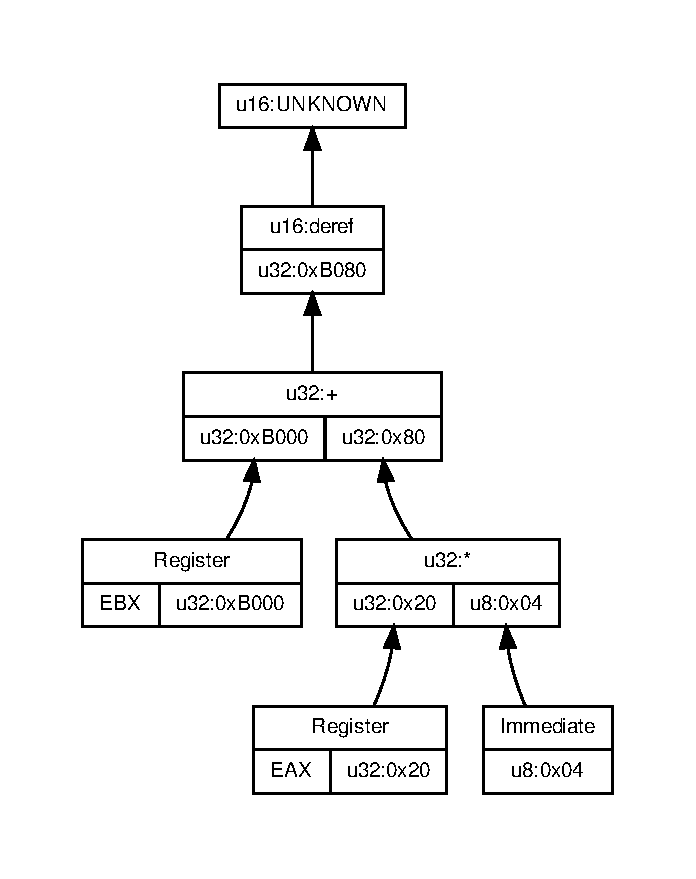
\includegraphics{fig/deref-eval}
\caption{Applying \code{eval} to a Dereference tree with two registers
having user-provided values.}
\label{fig:deref-eval}
\end{figure}

\begin{apient}
typedef boost::shared_ptr<Expression> Ptr
\end{apient}
\apidesc{
    A type definition for a reference-counted pointer to an \code{Expression}.
}

\begin{apient}
bool operator==(const Expression &rhs) const  
\end{apient}
\apidesc{
Compare two AST nodes for equality.

Non-leaf nodes are equal if they are of the same type and their children are
equal. \code{RegisterAST}s are equal if they represent the same register.
\code{Immediate}s are equal if they represent the same value.
}

\begin{apient}
virtual void getUses(set<Expression::Ptr> & uses)
\end{apient}
\apidesc{
    The use set of an \code{Expression} is defined as follows:
    \begin{itemize}
    \item A \code{RegisterAST} uses itself
    \item A \code{BinaryFunction} uses the use sets of its children
    \item A \code{Immediate} uses nothing
    \item A \code{Dereference uses the use set of its child}
    \end{itemize}

    The use set of this node is appended to the set \code{uses}.
}

\begin{apient}
virtual bool isUsed(Expression::Ptr findMe) const
\end{apient}
\apidesc{
    Unlike \code{getUses}, \code{isUsed} looks for \code{findMe} as a subtree of
    the current tree. \code{getUses} is designed to return a minimal set of
    registers used in this tree, whereas \code{isUsed} is designed to allow
    searches for arbitrary subexpressions. \code{findMe} is the AST node to find
    in the use set of this node. 

    Returns \code{true} if \code{findMe} is used by this AST node.
}

\begin{apient}
virtual std::string format(formatStyle how == defaultStyle) const
\end{apient}
\apidesc{
    The \code{format} interface returns the contents of an \code{Expression}
    object as a string. By default, \code{format} produces assembly language.
}

\begin{apient}
const Result & eval() const
\end{apient}
\apidesc{
    If the \code{Expression} can be evaluated, returns a \code{Result}
    containing its value. Otherwise returns an undefined \code{Result}.
}

\begin{apient}
const setValue(const Result & knownValue)
\end{apient}
\apidesc{
    Sets the result of \code{eval} for this \code{Expression} to
    \code{knownValue}.
}

\begin{apient}
void clearValue()
\end{apient}
\apidesc{
    \code{clearValue} sets the contents of this \code{Expression} to undefined.
    The next time \code{eval} is called, it will recalculate the value of the
    \code{Expression}.
}

\begin{apient}
int size() const
\end{apient}
\apidesc{
    \code{size} returns the size of this \code{Expression}'s \code{Result}, in
    bytes.
}

\begin{apient}
bool bind(Expression * expr, const Result & value)
\end{apient}
\apidesc{
    \code{bind} searches for all instances of the Expression \code{expr} within
    this Expression, and sets the result of \code{eval} for those subexpressions
    to \code{value}. \code{bind} returns \code{true} if at least one instance of
    \code{expr} was found in this Expression.

    \code{bind} does not operate on subexpressions that happen to evaluate to
    the same value. For example, if a dereference of \code{0xDEADBEEF} is bound
    to 0, and a register is bound to \code{0xDEADBEEF}, a deference of that
    register is not bound to 0.
}

\begin{apient}
virtual void apply(Visitor *)
\end{apient}
\apidesc{
    \code{apply} applies a \code{Visitor} to this \code{Expression}. Visitors
    perform postfix-order traversal of the ASTs represented by an
    \code{Expression}, with user-defined actions performed at each node of the
    tree. We present a thorough discussion with examples in Section
    \ref{sec:visitor}. 
}

\begin{apient}
std::vector<Expression::Ptr> getSubexpressions() const
\end{apient}
\apidesc{
Returns all subexpressions used by the current expression.
}
